\experiment{File Allocation Strategies}{11/10/2023}

\section{Aim}
Simulate file allocation strategies. a) Sequential b) Linked c) Indexed .

\section{Algorithm}

\subsection{Sequencial}
\begin{enumerate}[label=\arabic*.]
    \item Start
    \item Enter the user to enter the number of blocks.
    \item Initialize all elements of the block array to 0.
    \item As long as there are more files to allocate:
    \begin{enumerate}[label=4.\arabic*.]
        \item Set flag to 0.
        \item Enter the starting block of the file $b$.
        \item Enter the length of the file $l$.
        \item If $l > n$ then print "File cannot be allocated due to insufficient space in the disk" and go to step 5.
        \item Else set $k$ to 0.
        \item Check if the current block is already allocated then set flag to 1 and break the loop.
        \item If flag is 0 allocate the blocks.
        \item Print the allocated blocks.
    \end{enumerate}
    \item Stop.
\end{enumerate}

\subsection{Linked}
\begin{enumerate}[label=\arabic*.]
    \item Start
    \item Enter the user to enter the number of blocks.
    \item Initialize all elements of the block array to 0.
    \item As long as there are more files to allocate:
    \begin{enumerate}[label=4.\arabic*.]
        \item Set flag to 0.
        \item Enter the starting block of the file $b$.
        \item Enter the length of the file $l$.
        \item If starting block is already allocated then print "starting block is allocated" and go to step 5.
        \item Else set $k$ to 0.
        \item Create a new block struct pointer $b$.
        \item Set $b \rightarrow block\_no$ to $ptr \rightarrow start\_block$.
        \item Set $b \rightarrow next$ to NULL.
        \item Set $ptr \rightarrow list$ to $b$.
        \item Set $blocks[ptr \rightarrow start\_block]$ to 1 to mark it as allocated.
        \item Set count to 1.
        \item Set $i$ to $ptr \rightarrow start\_block + 1$.
        \item If $i < ptr \rightarrow length$:
        \begin{enumerate}[label=(a)]
            \item If $i \geq n$ set $i$ to 0.
            \item If the current block is not allocated create a new block struct pointer and set $new\_block \rightarrow block\_no$ to $i$ and $new\_block \rightarrow next$ to NULL.
            \item Assign the link and increment $i$ and go to step 4.13.
        \end{enumerate}
        \item If count is less than $ptr \rightarrow length$, print "Allocation not possible due to insufficient storage!".
        \item Print the allocated blocks.
    \end{enumerate}
    \item Stop.
\end{enumerate}

\subsection{Indexed}
\begin{enumerate}[label=\arabic*.]
    \item Start
    \item Enter the user to enter the number of blocks.
    \item Initialize all elements of the block array to 0.
    \item As long as there are more files to allocate:
    \begin{enumerate}[label=4.\arabic*.]
        \item Set count to 0.
        \item Enter the index block number of the file $index$.
        \item If $index \geq n$ or $index < 0$, then print "Invalid index block number".
        \item If the index block is already allocated print "Index block already allocated".
        \item Enter the user to enter the length of the file.
        \item Mark the index block as allocated.
        \item Initialize start to 0.
        \item while $i < ptr \rightarrow length$:
        \begin{enumerate}[label=(a)]
            \item If the current block is not allocated, set the block as allocated.
            \item Increment count by 1.
        \end{enumerate}
        \item If count $<$ length, print "Insufficient storage! No allocation.".
        \item Print the allocated blocks.
    \end{enumerate}
    \item Stop
\end{enumerate}


\section{C Program}

\subsection{Sequencial}
\begin{lstlisting}[label={list:c_program:queue}]
#include <stdio.h>

void main() {
    int n, b, l, k, flag, block[100];
    char c = 'y';

    printf("No of blocks: ");
    scanf("%d", &n);

    for (int i = 0; i < n; i++)
        block[i] = 0;

    while (c == 'y' || c == 'Y') {
        flag = 0;
        printf("Enter file starting block: ");
        scanf("%d", &b);
        printf("Enter file length: ");
        scanf("%d", &l);

        if (l > n)
            printf("File cannot be allocated!!\nInsufficient space in the disk.\n");
        else {
            k = 0;
            for (int j = b; j < b + l; j++) {
                if (block[j] == 1) {
                    flag = 1;
                    break;
                }
            }

            if (flag == 0) {
                printf("File allocated to blocks: ");
                for (int j = b; j < b + l; j++) {
                    block[j] = 1;
                    printf("%d ", j);
                }
                printf("\n");
            } else
                printf("File cannot be allocated!!\nSome blocks are already allocated.\n");
        }
        printf("\nAre there more files? (y/n): ");
        scanf(" %c", &c);
    }
}
\end{lstlisting}
\subsection{Linked}
\begin{lstlisting}[label={list:c_program:queue}]
#include <stdio.h>
#include <stdlib.h>

struct block {
    int block_no;
    struct block *next;
};

struct file {
    int start_block;
    int length;
    struct block *list;
};

void main() {
    int n, blocks[100], flag = 0, count, i;
    char c = 'y';

    printf("Enter the number of free blocks: ");
    scanf("%d", &n);

    for (int i = 0; i < n; i++)
        blocks[i] = 0;

    while (c == 'y' || c == 'Y') {
        struct file *ptr = (struct file *)malloc(sizeof(struct file));
        
        printf("Enter file starting block: ");
        scanf("%d", &(ptr->start_block));
        
        printf("Enter file length: ");
        scanf("%d", &(ptr->length));

        if (blocks[ptr->start_block] == 1) {
            printf("Starting block already allocated! Allocation not possible.\n");
        } else {
            struct block *b = (struct block *)malloc(sizeof(struct block));
            b->block_no = ptr->start_block;
            b->next = NULL;
            ptr->list = b;
            blocks[ptr->start_block] = 1;
            count = 1;
            i = ptr->start_block + 1;

            while (count < ptr->length) {
                if (i >= n)
                    i = 0;

                if (blocks[i] == 0) {
                    struct block *new_block = (struct block *)malloc(sizeof(struct block));
                    new_block->block_no = i;
                    new_block->next = NULL;

                    struct block *p = ptr->list;
                    while (p != NULL && p->next != NULL)
                        p = p->next;

                    p->next = new_block;
                    count++;
                    blocks[i] = 1;
                }
                i++;
            }

            if (count < ptr->length) {
                printf("Allocation not possible due to insufficient storage!\n");
            } else {
                printf("File allocated to disk.\n");
                printf("Linked list of blocks allocated to this file: ");
                struct block *p = ptr->list;
                while (p->next != NULL) {
                    printf("%d->", p->block_no);
                    p = p->next;
                }
                printf("%d", p->block_no);
            }
        }
        printf("\nAre there more files? (y/n): ");
        scanf(" %c", &c);
    }
}
\end{lstlisting}

\subsection{Indexed}
\begin{lstlisting}[label={list:c_program:queue}]
#include <stdio.h>
#include <stdlib.h>

void main() {
    int n, blocks[100], flag = 0, index, length, count = 0, index_block[100];
    char c = 'y';

    printf("Enter the number of blocks: ");
    scanf("%d", &n);

    for (int i = 0; i < n; i++)
        blocks[i] = 0;

    while (c == 'y' || c == 'Y') {
        count = 0;

        printf("Enter file index block number: ");
        scanf("%d", &index);

        if (index >= n || index < 0) {
            printf("Invalid index block number! Please enter a valid index.\n");
            continue;
        }

        if (blocks[index] == 1) {
            printf("Index block already allocated! No allocation possible.\n");
        } else {
            printf("Enter file length: ");
            scanf("%d", &length);
            blocks[index] = 1;
            int start = 0;

            for (int i = start; i < n && count < length; i++) {
                if (blocks[i] == 0) {
                    blocks[i] = 1;
                    index_block[count] = i;
                    count++;
                }
            }

            if (count < length) {
                printf("Insufficient storage! No allocation.\n");
                blocks[index] = 0;

                for (int i = start; i < n && i < start + count; i++)
                    blocks[i] = 0;
            } else {
                printf("File allocated to disk with index block %d\n", index);
                
                for (int i = 0; i < count; i++)
                    printf("%d->%d\n", index, index_block[i]);
            }
        }
        printf("\nAre there more files? (y/n): ");
        scanf(" %c", &c);
    }
}
\end{lstlisting}


\section{Output}
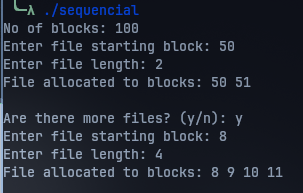
\includegraphics[]{Cycle_4//Outputs/sequential.png}
\newline
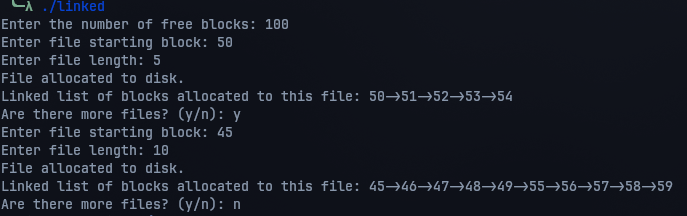
\includegraphics[width=0.95\linewidth]{linked1.png}
\newline
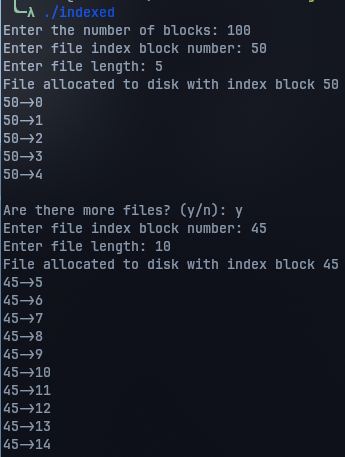
\includegraphics[]{Cycle_4//Outputs/indexed.png}




\section{Result}
Executed file allocation strategies successfully.